%%
%% DataTypes.tex
%% Login : <hoang-trong@hoang-trong-laptop>
%% Started on  Fri Jun 12 19:41:09 2009 Hoang-Trong Minh Tuan
%% $Id$
%% 
%% Copyright (C) 2009 Hoang-Trong Minh Tuan
%% This program is free software; you can redistribute it and/or modify
%% it under the terms of the GNU General Public License as published by
%% the Free Software Foundation; either version 2 of the License, or
%% (at your option) any later version.
%% 
%% This program is distributed in the hope that it will be useful,
%% but WITHOUT ANY WARRANTY; without even the implied warranty of
%% MERCHANTABILITY or FITNESS FOR A PARTICULAR PURPOSE.  See the
%% GNU General Public License for more details.
%% 
%% You should have received a copy of the GNU General Public License
%% along with this program; if not, write to the Free Software
%% Foundation, Inc., 59 Temple Place, Suite 330, Boston, MA 02111-1307 USA
%%

\chapter{Data Types (Objects)}
\label{chap:data-types}

\section{Introduction}
\label{sec:introduction}


For permanent storage, data should be stored as files in hard
drives. However, in order to analyze data, it should be read into
memory. The methods to read data from files are discussed in another
\hyperref[chap:files]{chapter}. In this chapter, we will mainly discuss
how to manipulate the objects in different data types.
To completely define an object, it needs a type and a mode. 

\subsection{Type}
\label{sec:type}

R language provides a safe way to access data via symbolic names
called objects (or variables). Each object belongs to a specific (R
internal) {\bf type} which can be determined by using the
{\bf typeof()} command.

\begin{lstlisting}
typeof(object)
\end{lstlisting}
RETURN a character string whose content is an item in the structure
'TypeTable' in 'src/main/util.c'. 


The current possible types are: {\it logical}, {\it integer}, {\it double},
{\it complex}, {\it character}, {\it raw} and {\it list}, {\it NULL},
{\it closure} (for function), special and builtin (basic functions
and operators), {\it environment}, {\it S4} (some S4 objects) and others
that are unlikely to be seen at user level ({\it symbol, pairlist,
promise, language, char, ..., any, expression,
externalptr, bytecode} and {\it weakref}).

\begin{lstlisting}
"NULL"         NULL
"symbol"       a variable name
"pairlist"     a pairlist object (mainly internal)
"closure"      a function
"environment"  an environment
"promise"      an object used to implement lazy 
                  evaluation
"language"     an R language construct
"special"      an internal function that does not 
                  evaluate its arguments
"builtin"      an internal function that evaluates 
                  its arguments
"logical"      a vector containing logical values
"integer"      a vector containing integer values
"double"       a vector containing real values
"complex"      a vector containing complex values
"character"    a vector containing character values
"any"          a special type that matches 
                   all types: there are no 
                   objects of this type
"expression"   an expression object
"list"         a list
"externalptr"  an external pointer object
"weakref"      a weak reference object
"raw"          a vector containing bytes
"S4"           an S4 object which is not 
                   a simple object
"bytecode"     byte code (internal only) ***
"..."          the special variable length 
                   argument ***
"char"         a scalar string object 
                  (internal only) ***
\end{lstlisting}
Objects of types marked with a *** are not intended to be manipulated
by users.

\subsection{Mode}
\label{sec:mode}

Besides its {\it type}, an object also have a {\bf mode}.  Modes have
the same set of names as \hyperref[sec:type]{types}, except
\begin{itemize}
\item integer, double \verb|->| mode: numeric

\item special, builtin \verb|->| mode: function

\item symbol \verb|->| mode:name

\item language \verb|->| mode: ( or call
\end{itemize}

This is normally applied for object with data structure (e.g. vector,
array, matrix...) which is composed of fundamental constituents. We
use modes to determine such constituents: numeric, complex, logical,
character, list, function, call, expression, name, etc. A mode can be
accessed via {\bf mode()} function.

\begin{lstlisting}
mode(object)
\end{lstlisting}

You can change the mode of an object via
\begin{lstlisting}
mode(object) <- "newmode"
\end{lstlisting}
A more efficient internal version of {\it mode\verb|<-|} is storage.mode(x)\verb|<-|.
\subsection{Storage mode}
\label{sec:storage-mode}

{\bf storage.mode()} is a more efficient version of mode() command.
The mode of the returned object of a function is determined by the
{\bf storage.mode()} function. It can be: logical, integer, double,
complex, character, symbol etc

\begin{lstlisting}
storage.mode(object)
\end{lstlisting}

Here, we will discuss the most important objects, in alphabet
order. To test for the data type of an object, use {\bf class()}
function

\begin{lstlisting}
>> class(object)
\end{lstlisting}

\subsection{Attributes}
\label{sec:attributes}

Even though R language is not an object-oriented (OO) language, every
object can have one or more attributes. The concept of attributes
refers to any of its property which can be of intrinsic or
user-defined, e.g.

\begin{itemize}
\item mode: see above. an intrinsic attribute

\item length: number of (highest level) elements; an intrinsic
  attribute

\item dim: used to implement arrays, matrices, data.frames

\item names: used to label the elements of a vector (/array) or list,
  or the variables of a data frame. (For one-dimensional arrays,
  dimnames[[1]] is accessed.)

\item dimnames: list of character vectors used to label the dimensions
  of an array, matrix, or a data.frame.

\item class: vector of character strings (``class names'') used for OO
  programming, e.g.  data.frame, c('ordered', 'factor') or table

\item  tsp: used for periodic time series

\item levels: for factors; of type character

\item  contrasts: for factors

\item  row.names: to label the cases of a data frame

\item  rownames/colnames: first dimnames; = row.names/names in a data frame

\item source: the source code of user defined functions

\item comment: is handled by the function comment()

\end{itemize}

\subsection{Levels}
\label{sec:levels}

An object can have elements at different levels. For example a list
whose elements are lists.
\begin{lstlisting}
z1 = c (14,5,2)
z2 = c (1 , 3, 4)
z = c (z1,z2)
\end{lstlisting}
So, $z1,z2$ are two elements at the highest level of $z$ while
$14,5,2,1,...$ are elements at a lower level.

\subsection{Associated functions}
\label{sec:associated-functions}

There are various functions to set/get these modes/types/attributes.

\begin{itemize}
\item typeof(), mode(), storage.mode(), attributes(), attr(),
  length(), dim(), names(), dimnames(), class(), tsp(), levels(),
  contrasts(), rownames(), row.names(), colnames(), 

  mostly returning a vector (a list for attributes()); comment()

\item vector(), matrix(), array(), factor(), ordered(), list(),
  data.frame(), function(), call(),expression() (note the difference
  to as.expression()), creating the respective object

\item 
\begin{lstlisting}
is.object(), is.vector(), is.array(), is.matrix(), 
is.factor(), is.ordered(), is.list(), 
is.data.frame(), is.function(), is.language(), 
is.call(), is.expression(), 
is.symbol() (=is.name()),is.null(), is.pairlist(), 
is.environment(), is.table(), is.ts(),
is.tskernel(), is.atomic(), is.recursive(), 
is.logical(), is.integer(), is.double(), 
is.real(), is.complex(), is.character(),
is.numeric(), is.na() (vectorized), 
is.nan() (vect.), is.finite(vect.), 
is.infinite (vect.): 
\end{lstlisting}
  returning logical vectors (mostly of length 1)

\item as.vector(), as.symbol() (=as.name()), as.numeric(),
  as.integer() etc, 

  attempting a coercion of objects/modes/types etc; unlist(). E.g.:
  \lstinline!x <- 1; eval(as.symbol(``x''))!
\end{itemize}

\subsection{Indexing}
\label{sec:indexing}

Several constructs in R are complicated structures that are composed
of elements. Individual elements and subsets can be accessed through
indexing operators. Indexing can be used to set/get, add/remove one or
more elements.

R has three basic indexing operators ([], [[]], \$) with syntax
displayed by the following examples

\begin{lstlisting}

     x[i]
     x[i, j]
     x[[i]]
     x[[i, j]]
     x$a
     x$"a"
\end{lstlisting}
The form [[...]] only accept a single index (integer or character),
while [...] can accept a vector.
\begin{lstlisting}
x[[4]]

x[c(2,4,1)]
\end{lstlisting}
The form \$ is applied to recursive objects (lists, pairlists) and
allows a string literal or a symbol as an index. It means that the
index cannot be an expression. Otherwise, [[expr]] has to be used.


\textbullet A vector: use [...]

\textbullet A list: use [[...]] to return a single element, [...] to
return a list of selected elements.

\textbullet In vectors, matrices: [[...]] is slightly different from
[...], as it drops any {\it names} and {\it dinames} attributes and
partial matching is used for character indices.

\textbullet (since R 2.6.0), \$ when applied to a non-recursive object
is an error.

For more detail of indexing, read the corresponding data types.

\section{Special objects}
\label{sec:special-objects}

\subsection{NULL}
\label{sec:null}

It is  used whenever there  is a need  to indicate or specify  that an
object is absent.  It should not be confused with a  vector or list of
zero  length.  

The NULL object has no type and no modifiable properties. There is
only one NULL object in R, to which all instances refer.  To test for
NULL use {\bf is.null()} function. You cannot set attributes on NULL.


\section{Array}
\label{sec:array}

Arrays are vector plus a {\it dim} attribute (dimension vector).  
Arrays are ordered-column major order.

R language supports ragged array, or jagged array in which the valid
range of one index depends on the value of another. Simply it means
that different rows have different sizes.

To manipulate data based on array margins, R provides a very powerful
function {\bf apply()} or {\bf lapply()} or {\bf sapply()}.
\begin{lstlisting}
apply(X, margin, FUN, ...)
\end{lstlisting}
where {\it margin} can be either 1, 2, or c(1,2). X is an array.
FUN is a function which can return either
\begin{enumerate}
\item a vector of length $n$, then apply() returns an array of
  dimension dim(n, dim(X)[margin])
\item a scalar, then apply() return a vector if margin is a single
  value.

\item a scalar, then apply() returns an array of dimension
  dim(X)[margin] if margin is a vector.
\end{enumerate}



\section{Boolean}
\label{sec:boolean}

\section{characters}
\label{sec:characters}


\chapter{Array/Matrix/Table-like data}


\section{data.frame}
\label{sec:data.frame}

A {\bf data.frame} is a matrix-like object in which different columns can be of
different types/\hyperref[mode]{modes}/attributes
(Sect.\ref{sec:data.frame-intro}).


Data frame also has {\it dim} attributes of length 2 (the first value is the
number of rows, the second one is the number of columns).


A data.frame usually have a {\it name} attribute for the variables
(columns) and {\it row.names} attribute for the cases (rows). 

A column is implemented as a list.  Rows and columns can have assigned
labels which can be retrieved using {\bf dimnames()} command.
\begin{lstlisting}
dimnames(data.frame)[[1]]
dimnames(data.frame)[[2]]
\end{lstlisting}
This is similar to SAS or SPSS datasets.

This data type is of particularly helpful for storing reading from
text files since spreadsheet data (from Excel …) are mostly of this
form. Here is a spreadsheet in a form of a data.frame.
\begin{figure}[htb]
  \centerline{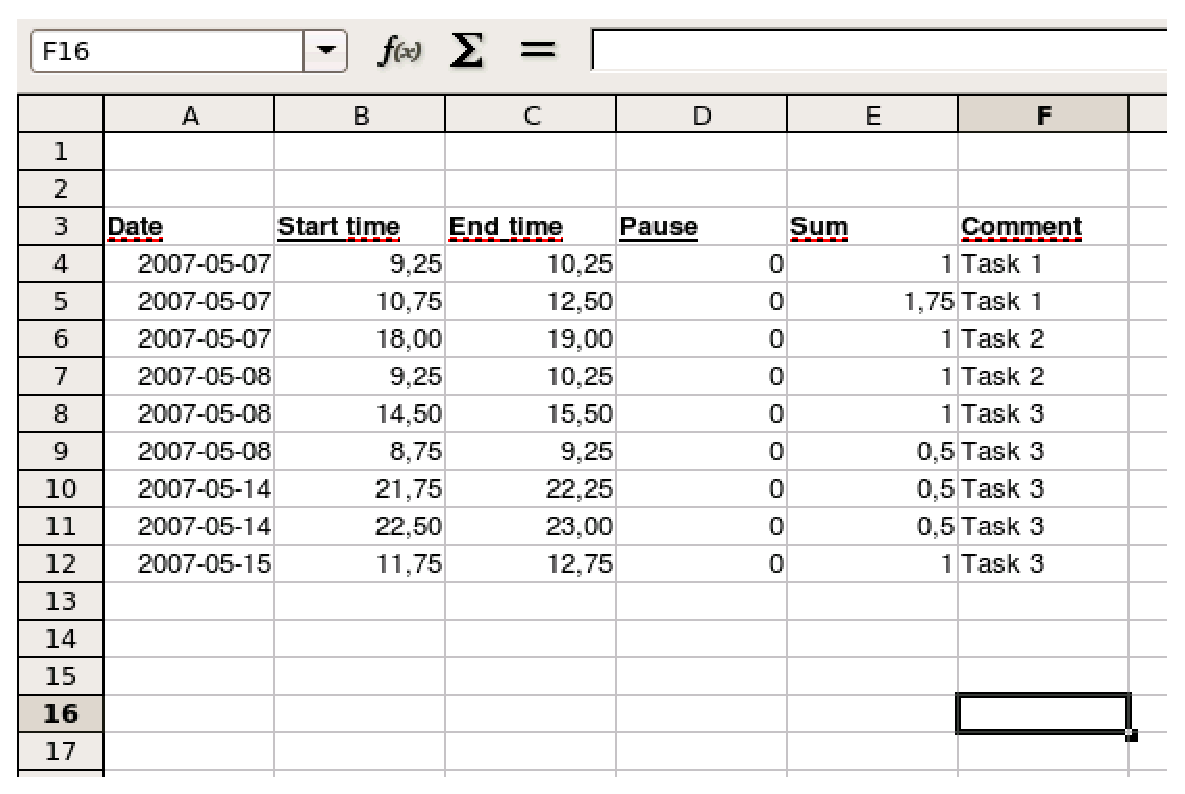
\includegraphics[height=7cm]{./images/data_frame.eps}}
  \caption{A spreadsheet}\label{fig:data_frame}
\end{figure}

Be reminding that the values of the response variable must appear on
the same column; other columns should be the value for the
corresponding independent variables. The Excel function called
{\it Pivot table} is helpful to map your data to be in the form of a
data.frame. In order for R to read the file, in Excel, you can save
the file in  'Text (Tab delimited)' format.

In fact, a data.frame is a list of variables of the same length with
unique row names. You can create a data.frame object by combining some vectors
\begin{lstlisting}
d <- c(1,2,3,4)
e <- c("red", "white", "red", NA)
f <- c(TRUE,TRUE,TRUE,FALSE)
mydata <- data.frame(d,e,f, row.names=c(4,3,'a12',5))
\end{lstlisting}

\begin{lstlisting}
data.frame(..., row.names = NULL, check.rows = FALSE,
           check.names = TRUE,
      stringsAsFactors = default.stringsAsFactors())
\end{lstlisting}
with
\begin{itemize}
\item row.names = an integer-vector giving the row names
\item check.rows = if you want each row has a unique name, set it to
  TRUE 
\item check.names = TRUE(by default), each column has a unique name.
\item stringsAsFactors = should character vectors be converted to
  Factors.  default.stringAsFactors() can be adjusted by setting
  options (stringsAsFactors = FALSE)
\end{itemize}

\subsection{Column names}
\label{sec:column-names}

Each column has its own name, to access the list of column's names you
can use {\bf names(data.frame)} or {\bf dimnames(data.frame)[[2]]}
command.

\begin{lstlisting}
>> names(mydata)
>> dimnames(mydata)[[2]]
\end{lstlisting}

The column's names can also be changed by assigning a new vector of
names to {\bf names(data.frame)}

\begin{lstlisting}
>> names(mydata) <- c("ID", "Color", "Passed")
\end{lstlisting}

\subsection{Retrieve data}
\label{sec:retrieve-data}


To access/retrieve item in an entire column, there are multiple ways
\begin{itemize}
\item use column label: \verb!data.frame$column_name!
\item use column index: \verb!data.frame[,index]!
\item use column label as column index: \verb!data.frame[column_name]!
\item exclude/remove a column by using negate value:
  \verb!data.frame[,-index]!
\end{itemize}

To access/retrieve any item (more general) from a data.frame of size
$m\times n$: since a data.frame is a column-based matrix-like data
structure, we can access

\begin{itemize}
\item the $i$-th element : \verb!data.frame[i]!

\item a range of element : \verb!data.frame[i:j]! with $0<i<j\le
  m\times n$ 

\item select all but one element $i$: \verb!data.frame[-i]!

\item slicing: including elements reside at arbitrary location
  (indicated by a vector): \verb!data.frame[c(i,j,k)]!

\item select items satisfied a logical operator:
  \verb!data.frame[data.frame > Z]! with $Z$ is any value that can be
  compared with items in the data.frame object

\item use the powerful function {\bf subset()} to select row-based
  items. RETURN: data.frame
\begin{lstlisting}
subset(x, subset, select, drop = FALSE, ...)
\end{lstlisting}
with
\begin{itemize}
\item x : either a vector, a matrix or a data.frame
\item subset : a logical expression indicating elements or rows to
    keep if the expression applied to that element (row) is TRUE
    (missing values are those that make the expression FALSE)
   
  \item select : an expression, indicating columns to select from a
    data frame or a matrix (NOT applied for vectors)
\end{itemize}
NOTE: column label can be used as variable in the expression 

\item use the {\bf with(data.frame, expr)} function: return a list of
  items in the data.frame that satisfy {\it expr}. {\it expr} is
  evaluated in a local environment constructed from data.frame
  (i.e. not in the user's workspace).
\end{itemize}

{\bf Example}:
\begin{lstlisting}
> airquality
    Ozone Solar.R Wind Temp Month Day
1      41     190  7.4   67     5   1
2      36     118  8.0   72     5   2
3      12     149 12.6   74     5   3
4      18     313 11.5   62     5   4
5      NA      NA 14.3   56     5   5
6      28      NA 14.9   66     5   6
7      23     299  8.6   65     5   7
8      19      99 13.8   59     5   8
9       8      19 20.1   61     5   9
    # select row entries from 2 columns (Ozone, Temp) 
    # with the Temp values > 80
> subset(airquality, Temp > 80, select = c(Ozone, Temp))
    # select all row entries (except entries from Temp column)
    # with Day == 1 
> subset(airquality, subset = (Day == 1), select = -Temp)
    # select all row entries (except entries from Temp column)
    # with Day > 1 and Wind < 10
> subset(airquality, subset = (Day > 1 & Wind < 10), select = -Temp)
    # select all row entries from columns 
    # starting from Ozone to Wind 
> subset(airquality, select = Ozone:Wind)
    # 
> with(airquality, subset(Ozone, Temp > 80))
\end{lstlisting}

Count the number of rows, we convert it to {\it table} data type and
use {\bf as.numeric()}
\begin{lstlisting}
X = subset(hospital,  select = c(V7,V8)) # data.frame with 2 columns

O11 = as.numeric(table(subset(X, V7 == 1 & V8 == 1)))
O12 = as.numeric(table(subset(X, V7 == 2 & V8 == 1)))
O21 = as.numeric(table(subset(X, V7 == 1 & V8 == 2)))
O22 = as.numeric(table(subset(X, V7 == 2 & V8 == 2)))

\end{lstlisting}

\section{Tibble}
\label{sec:tibble}

Tibble is a modern rethinking of R's data.frame (Sect.\ref{sec:data.frame}).


\section{factor}
\label{sec:factor}

In R, to handle nominal and ordered categorical data, a new concept
{\bf factor} is used. Example of nominal data is sex (male,
female). Example of ordered categorical data is severity of a disease
after the treatment (serious, mild, the same, better).

Each possible value of such type of data is a possible categorical
value (or level), rather than real characters or digits. Hence, a
factor in an object with a level (and optionally contrast)
attribute. Its class is {\it factor} implemented as an integer vector
with a mapped vector of names for the levels, e.g. (1,0) for (male,
female). Hence, {\it typeof(factor)} returns INTEGER,
{\it mode(factor)} returns NUMERIC.


So, the question is what it differs from category? - Factors have all
the features of categories, with some added class distinctions; in
particular, there is a distinction between factors and ordered
factors.

{\bf NOTE}: A factor with two possible values is said to be a
two-level factor.




\section{list (generic vector)}
\label{sec:list}

A list is a recursive structure, with type (Sect.\ref{sec:type}) and mode
(Sect.\ref{sec:mode}) are {\it list}. Their components can be of any type and
mode. Hence, a list is also called a {\it generic vector}.
\begin{lstlisting}
list(...)
\end{lstlisting}

Example: a list comprised of 3 vectors (Sect.\ref{sec:vector})
\begin{verbatim}
> n = c(2, 3, 5) 
> s = c("aa", "bb", "cc", "dd", "ee") 
> b = c(TRUE, FALSE, TRUE, FALSE, FALSE) 
> x = list(n, s, b, 3)   # x contains copies of n, s, b 
\end{verbatim}

A slice of a list contains one or more elements in a list.
With an index vector, we can retrieve a slice with multiple members.
\begin{verbatim}
> x[2] 
[[1]] 
[1] "aa" "bb" "cc" "dd" "ee" 

> x[c(2, 4)] 
[[1]] 
[1] "aa" "bb" "cc" "dd" "ee" 
 
[[2]] 
[1] 3 
\end{verbatim}

{\bf Direct member reference}:
Elements in a list is assessed via double bracket [[...]]] so that we can
modified it
\begin{verbatim}
> x[[2]]            # which is a vector
[1] "aa" "bb" "cc" "dd" "ee" 

> x[[2]][2]         # index the second element in the vector x[[2]]
\end{verbatim}

{\bf Named list members}: a member of a list can have a name so that it can be
referenced using name instead of the integer index.
\url{http://www.r-tutor.com/r-introduction/list/named-list-members}


\begin{lstlisting}
x[[1]] = 2
x[[2]] = c(4,2)
\end{lstlisting}


\section{matrix}
\label{sec:matrix}

A matrix is an array with {\it dim} attribute of length 2.


\textcolor{red}{Create a matrix from a vector} by casting a vector to
a matrix
\begin{lstlisting}
 matrix(data = NA, nrow = 1, ncol = 1, byrow = FALSE,
            dimnames = NULL)
\end{lstlisting}
with {\it data} is a vector. Elements in the vectors are filled in the
matrix in column-based (by default) or row-based (when byrow=TRUE).
\begin{lstlisting}
> m <- matrix(1:4, 2)
> m
          [,1] [,2]
     [1,]    1    3
     [2,]    2    4
> i <- matrix(c(1, 1, 2, 2), 2, byrow = TRUE)
> i
          [,1] [,2]
     [1,]    1    1
     [2,]    2    2
> m[i]
     [1] 1 4
\end{lstlisting}

\textcolor{red}{Create a matrix by combining old ones}: You can create
a new matrix by combining matrices/vectors in a column-wise manner or
row-wise manner using {\bf cbind(obj1, obj2...)} and {\bf rbind(obj1,
  obj2...)}, respectively. 

\begin{lstlisting}
rbind(matrix, vector1, vector2)
     # create a new matrix by adding two new vectors 
     # as two new rows

cbind(matrix, vector1, vector2)
     # create a new matrix by adding two new vectors 
     # as two new columns
\end{lstlisting}

\textcolor{red}{Transpose a matrix} use {\bf t(matrix)} function.

\textcolor{red}{Inverse matrix}: The inverse of a matrix, {\bf
  solve(matrix)} function 
\begin{lstlisting}
solve(A) ! A^{-1}
\end{lstlisting}

\textcolor{red}{Retrieve row/column size} use {\bf nrow(matrix)} and
{\bf ncol(matrix)} functions.

\textcolor{red}{Dot product} (element-by-element product) use *
\begin{lstlisting}
A * B
\end{lstlisting}

\textcolor{red}{Matrix product}, use \lstinline!%*%!
\begin{lstlisting}
C = A %*% B
\end{lstlisting}

\textcolor{red}{Cross-product} (matrix-vector product), use
\lstinline!t(A) %*% y! with $y$ is a vector,
and $A$ is a matrix. An alternative efficacy way is to use

\begin{lstlisting}
crossprod(A,y)
\end{lstlisting}

\textcolor{red}{Outer product}:  The outer product of two arrays X and Y
\begin{lstlisting}
Z = outer(X, Y, FUN="*", ...)

Z = X %o% Y
\end{lstlisting}
X and Y must be the first and second argument of the function
specified in FUN tag, any arguments specified in ... will be the
arguments in the function specified in FUN tag.  The dimension of Z
will be c(dim(X), dim(Y)).

\textcolor{red}{Diagonal entries}: Get the main diagonal entries in
the form of a vector, {\bf diag(matrix)} function.

\begin{lstlisting}
vect = diag(A)
\end{lstlisting}
This function can be used in different context.

\begin{lstlisting}
diag(vect) # return a diagonal matrix with its diagonal entries is
specified in vector vect

diag(k)    # return a k-by-k identity matrix (k is a numeric scalar)
\end{lstlisting}


\textcolor{red}{Linear equation}: Solving linear equations: $A.x = b$
with $x$ is a vector of unknown parameters
\begin{lstlisting}
x = solve(A, b)
\end{lstlisting}
Numerically, the inefficient and potentially unstable way is
\lstinline! x = solve(A) %*% B!.

\textcolor{red}{Quadratic form}: The quadratic form $x.A^{-1}x$ should
be computed using
\begin{lstlisting}
result = x %*% solve(A,x)
\end{lstlisting}


\section{numeric}
\label{sec:numeric}

\section{scalars}
\label{sec:scalars}

Scalars are treated as \hyperref[sec:vector]{vectors} of length 1.

\section{table}
\label{sec:table}

\section{vector}
\label{sec:vector}

\begin{lstlisting}
x = c(4,2,15,5,12.1)

x = c(a = 4, b=3, 23)
\end{lstlisting}

A vector can be thought of as contiguous cells containing data whose
elements must be of the same type, i.e. elements in a vector should
all belong to one of the 6 types: logical, integer, double, complex,
character and raw, with certain associated {\it modes} and
{\it storage modes}.

\begin{table}[hbt]
 \begin{center}
\caption{Terminology}
  \begin{tabular}{ccc}
    \hline
type & mode & storage.mode \\
    \hline\hline
logical & logical & logical \\
integer &  numeric & integer \\
double & numeric & double \\
complex & complex & complex \\ 
character & character & character \\
raw & raw & raw \\
  \end{tabular}
\end{center}
\label{tab:vector_prop}
\end{table}

A single element of a character vector is often referred to as a
{\it character string}.  To define a vector we only need to specify
its mode.



\textcolor{red}{Create a vector} of given length and mode
\begin{lstlisting}
>> x = vector(mode = "logical", length = 10) # return a new object
\end{lstlisting}

\textcolor{red}{Create a vector} by means of {\bf c()}  (combine,
concatenate) function
\begin{lstlisting}
x = c(1,3,4)
\end{lstlisting}

\textcolor{red}{Create a vector} by means of {\bf seq()} function, or
abbreviated as a colon (:)
\begin{lstlisting}
x = 1:5
x = seq(1,5,.3)
\end{lstlisting}

\textcolor{red}{Create a vector} by means of {\bf rep()} (repetitive)
function.
\begin{lstlisting}
>> x = rep(1:5, each=2)  # repeat each element twice
>> x
[1] 1 1 2 2 3 3 4 4 5 5
\end{lstlisting}

\textcolor{red}{Create a vector of NA values}: Indexing with a NA
value results to a vector of the same length with all elements are NA
values, except for the case NA is a part of the indexing vector.
\begin{lstlisting}
y = x[NA] # y = (NA, NA, NA, NA, NA)

y = x[c(1,NA)] # y = (4, NA)
\end{lstlisting}

\textcolor{red}{Create an empty vector}: Indexing with a zero value
results to an empty vector.

\textcolor{red}{Is a vector}: Check if a given variable is a vector of
specified mode
\begin{lstlisting}
is.vector(x, mode = "numeric")  # return TRUE/FALSE
\end{lstlisting}


{\bf IMPORTANT}: Don't use is.vector() at all at least not until we
[and the S authors?]  know what is desired?  Instead, use
\begin{verbatim}
		is.list()
and/or		is.atomic()  is.recursive()  is.array()
\end{verbatim}

\textcolor{red}{Length of a vector}: we use {\bf length(vector)}
function. 

\begin{lstlisting}
length(x)
\end{lstlisting}


\textcolor{red}{Map to a vector}: Coerce a given variable to the type
of vector of a specified mode
\begin{lstlisting}
as.vector(x, mode = "any")       # return a vector
\end{lstlisting}

\textcolor{red}{Access elements}: Using indexing [...] to access an
element

\begin{itemize}
\item If index is a non-integer, it is truncated to the closest
  integer less than it before use
\begin{lstlisting}
x[4.2] # x[4]
\end{lstlisting}

\item If index is a positive integer: select the element with that
  index
\begin{lstlisting}
x[c(4, 1)] 
\end{lstlisting}
If the index is positive and out of range, return NA value.

\item If index is a negative integer: select all elements except those
  indicated are selected
\begin{lstlisting}
x[c(-4, -1)] 
\end{lstlisting}
If the index is negative and out of range, it's an error

\item A logical vector of the same length can be used to specify which
  elements to be selected (TRUE)
\begin{lstlisting}
x[c(T, F, F, T, T)] # (4,12.1)
\end{lstlisting}
  If the logical vector is of shorter length, the elements will be
  recycled
\begin{lstlisting}
x[c(T,F)]  # x[c(T,F,T,F,T)]
\end{lstlisting}
  If the logical vector is of longer length, then the vector object is
  extended first before its elements are selected
\end{itemize}

\textcolor{red}{Remove attributes}: Drop all attributes, except
{\it names} and in multi-dimensional array, {\it dim} and
{\it dimnames} properties
\begin{lstlisting}
y = x[]
\end{lstlisting}


Elements in R language can have associated names ({\it names}
attribute).


\section{pairlist}
\label{sec:pairlist}

Pairlist objects are similar to Lisp's dotted-pair lists. Pairlist is
used extensively in R internal, but rarely visible in R interpreted
code. 

Pairlists are handled in the R language in exactly the same way as
generic vectors ('list'). In particular, elements are accessed
using [[...]]. Further, when an internal pairlist is accessed from R
it is generally (including when subsetted) converted to a generic
vector.

The use of pairlist is deprecated since generic vector (list) is more
efficient to use. A pairlist can be coerced to a generic vector.

%%% Local Variables: 
%%% mode: latex
%%% TeX-master: "R_language"
%%% End: 
